\chapter[Capítulo 4. Propuesta]{Propuesta}

\section{Introducción}

Una vez conocemos el funcionamiento, características, algunas formas de implementación y los problemas a los que se enfrentan cada una de las técnicas descritas hasta ahora (árboles de decisión, data streaming y la aplicación de restricciones monotónicas), procedemos a exponer la propuesta hacia la cual se encauza el propósito de este documento.\\

Hemos comprobado que existen métodos eficientes de adquisición de conocimiento y predicción sobre flujos de datos utilizando árboles de decisión, tales como Option trees y Hoeffding Anytime Tree (HATT), ambos basados en Hoeffding Tree, o incluso su versión mejorada para la detección del cambio de concepto en el tiempo (CVFDT).\\

Así mismo, hemos observado también que existen ejemplos de conjuntos de datos que poseen características dignas de ser tenidas en cuenta a la hora de crear un modelo de aprendizaje de conocimiento, ya que aportan una base de información subyacente a los datos que ofrece al algoritmo la capacidad de crear una estructura de datos más eficiente para la resolución de cualquier problema que se enfrente a datos de este estilo. Evidentemente hablamos de los conjuntos de datos que aguardan en sí una relación de monotonía entre los valores de los atributos de sus instancias y las clases asignadas a estas.\\

Tal como se muestra en \cite{ref14}, existen multitud de problemas en la vida diaria que requieren ser tratados como problemas de clasificación monotónica con el fin de ser correctamente resueltos. Este es el caso de aquella universidad que no quiera admitir a un solicitante con ciertas notas y rechazar a otro con notas iguales o más altas por no haber tenido en cuenta la monotonicidad del asunto, o el caso de una compañía de seguros de vida que no desea que sus decisiones dependan de un árbol de decisión que no tenga en cuenta que un solicitante anciano y poco saludable ha de cotizar una tasa de prima más alta que un solicitante joven y saludable. Otros problemas pueden ser los de credit scoring, elección de consumidor, selección de escuela y transporte, etc.\\

En el siguiente ejemplo veremos las consecuencias que puede tener el hecho de crear un árbol de clasificación no-monotónico en un problema de credit scoring simple. Los atributos utilizados en cada árbol son los ingresos(income) + los activos(assets) y los activos a solas respectivamente. 


\begin{figure}[H]
	\centering
	\begin{minipage}{0.47\textwidth}
		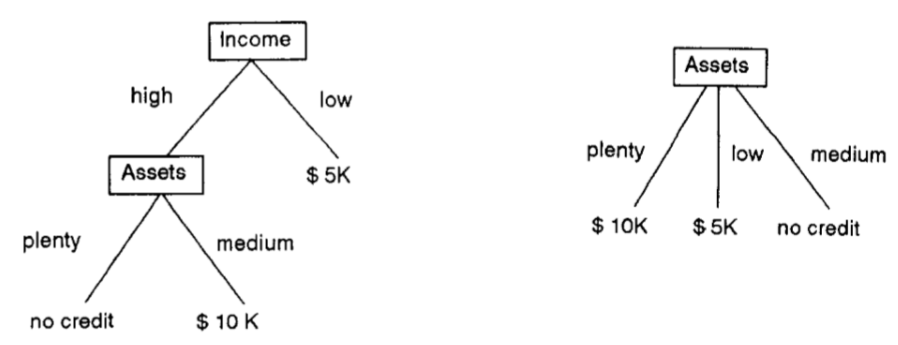
\includegraphics[width=1\textwidth]{imagenes/ejAr}
		\label{fig:a}
	\end{minipage}
	\hspace{5mm}
	\begin{minipage}{0.47\textwidth}
		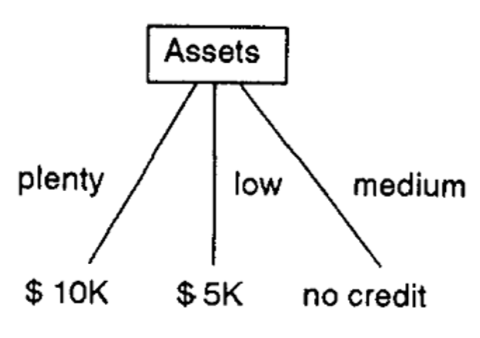
\includegraphics[width=1\textwidth]{imagenes/ejAr2}
		\label{fig:b}
	\end{minipage}
	\caption{Árboles no monotónicos\cite{ref14}}
\end{figure}

Como vemos, ambos árboles, al no poseer restricciones de monotonicidad, carecen también de sentido, ya que a un cliente con pocos activos se le autoriza una linea de crédito de cinco mil dólares, mientras que a un cliente con más activos no se le ofrece crédito alguno, por ejemplo.\\

El árbol no-monotónico de la derecha en la figura anterior, es el resultado surgido del siguiente conjunto de datos que \textbf{sí} guarda relación de monotonía entre los valores de los atributos y las clases asignadas. Tal como vemos, el hecho de que los datos sí sean monotónicos no asegura que el árbol creado a partir de él lo sea.\\
Los datos utilizados para ello son los siguientes:

\begin{figure}[H]
	\centering
	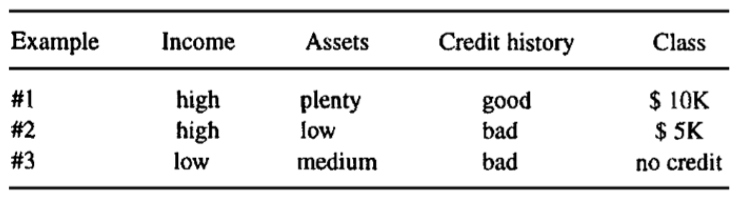
\includegraphics[width=0.9\textwidth]{imagenes/tablaEj} 
	\caption{Conjunto de datos monotónico\cite{ref14}}
\end{figure}

\section{Propuesta y resultados esperados}

Visto todo esto, parece lógico crear una adaptación de los algoritmos de árboles de decisión para data streaming que además posean información sobre restricciones de monotonía para conseguir resultados superiores en cuanto al análisis del dominio del problema al que se enfrentan los algoritmos que trabajan con este tipo de conjuntos de datos.\\

La propuesta no pretende conseguir resultados mejores en cuanto al accuracy obtenido en la predicción de resultados si no que, pretende que las estructuras creadas por los árboles de decisión para flujos de datos sean más fieles a la realidad que subyace bajo data sets con cierto nivel de monotonía en su relación atributos-clase, es decir, que se creen estructuras con sentido lógico, en lugar de árboles de decisión que obtengan buenos resultados en precisión pero malos en el concepto del dominio real que maneja el problema, lo que nos lleva a conseguir árboles con poca o nula interpretabilidad a la hora de la verdad.\\

Dicho esto, podría darse el caso en el que el algoritmo básico comparativo sin restricciones de monotonía aplicadas alcance un accuracy superior al que puedan alcanzar las adaptaciones realizadas las cuales si posean información sobre dichas relaciones monotónicas, por lo que, aunque también mediremos el nivel de acierto evidentemente, el objetivo principal de las mejoras a realizar con los novedosos algoritmos es conseguir un nivel mayor de monotonicidad y, por tanto, de lógica en el análisis del problema por parte de nuestros algoritmos, lo que les proporcionará un nivel de conocimiento superior del problema al que se están enfrentando.\\

Continuando con el ejemplo del credit scoring, a continuación veremos el árbol generado por un algoritmo que sí hace uso de información monotónica a la hora de su construcción. Se ve de forma rápida en esta figura que la lógica está presente en la resolución del problema.

\begin{figure}[H]
	\centering
	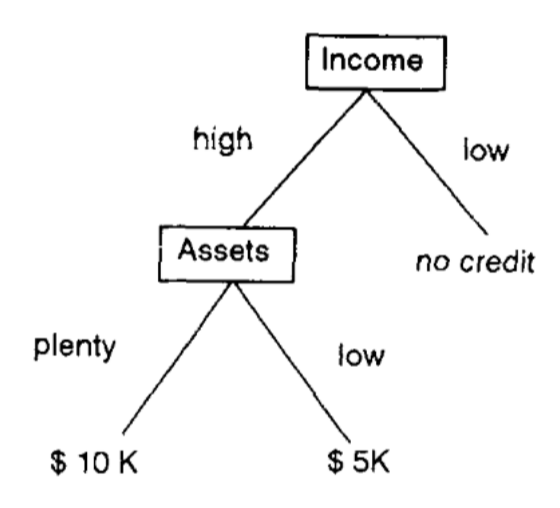
\includegraphics[width=0.55\textwidth]{imagenes/arbolBueno} 
	\caption{Árbol creado con restricciones monotónicas sobre\cite{ref14}}
\end{figure}

\section{Algoritmos a comparar}

Como \textbf{algoritmo de comparación} utilizaremos aquél del cual la literatura ha hecho más uso para la realización de estudios comparativos y mejoras de otros aspectos, es decir: \textbf{Hoeffding Tree}, la base de la que parten gran cantidad de algoritmos de árboles de decisión para el tratamiento de data streaming.\\

Los \textbf{algoritmos que pretenden hacerle frente} en cuanto a los aspectos ya mencionados serán:
\begin{itemize}
	\item Adaptación de Hoeffding Tree con restricciones monotónicas mediante el uso del \textbf{método basado en matriz}.
	\item Adaptación de Hoeffding Tree con restricciones monotónicas mediante el uso del \textbf{método de evaluación de monotonicidad de ramas}.
	\item Adaptación de Hoeffding Tree con restricciones monotónicas mediante el uso de\textbf{ ambos métodos al mismo tiempo}.
\end{itemize}











\newpage


